%% Standalone supplementary material: FEniCSx cross-code consistency check of collapsibleChannel.
%% DRAFT. Build (from this directory):  latexmk -pdf supplement_fenicsx_collapsiblechannel.tex
%% It does not read article.aux (no cross-references to the main article), so it builds on its own.
%% Bibliography key Baratta2023 (DOLFINx) is added to bibliography.bib byte-identically by the open draft PRs #69 and #70 and by this branch; PETSc, MUMPS:1, MUMPS:2, Heil2006 are already in bibliography.bib.
%% Data, scripts and provenance: paper-data/fenicsx_collapsiblechannel/ (README.md there).
\documentclass[sn-mathphys,Numbered]{sn-jnl}
\usepackage{graphicx}
\usepackage{amsmath,amssymb,amsfonts,bm}
\usepackage{xcolor}
\usepackage{soul}
\usepackage{manyfoot}
\usepackage{booktabs}
\usepackage{siunitx}
\usepackage{float}
\usepackage[utf8]{inputenc}
\usepackage[onehalfspacing]{setspace}
\usepackage{placeins}
\usepackage{geometry}
\geometry{a4paper,textwidth=15cm,textheight=24cm}
\setlength{\parskip}{0.5\baselineskip}
\raggedbottom

%% S-prefixed numbering
\renewcommand{\thesection}{S\arabic{section}}
\renewcommand{\thefigure}{S\arabic{figure}}
\renewcommand{\thetable}{S\arabic{table}}
\renewcommand{\theequation}{S\arabic{equation}}

\newcommand{\todo}[1]{\par\noindent\textcolor{red}{\rule{\linewidth}{0.8pt}}\par\nopagebreak
	\noindent{\small\color{red!70!black}\textbf{AUTHOR NOTE:} #1\par}\nopagebreak
	\noindent\textcolor{red}{\rule{\linewidth}{0.8pt}}\par}
%% Qualifier carried by every agreement statement.
\newcommand{\uref}{{\small[$U_\mathrm{ref}=0.30\,\%$ of the peak $P$; beam-versus-continuum model form unresolved]}}
\newcommand{\legbc}{\textcolor{red!70!black}{(legacy, pre-\#671)}}
\newcommand{\pP}{\ensuremath{\,\%\,P}}
%% run-in paragraph headings (the class default sets them on their own line with large skips)
\makeatletter
\renewcommand{\paragraph}[1]{\par\vspace{0.3\baselineskip}\noindent\textbf{#1}\ }
\makeatother

\begin{document}

\title[Supplementary material: FEniCSx collapsibleChannel]{Supplementary material: a same-lineage cross-code check of collapsibleChannel with a monolithic FEniCSx implementation}

\author*[1]{\fnm{Author} \sur{Placeholder}}\email{corresponding.author@example.org}
\author[1]{\fnm{Author} \sur{Placeholder 2}}

\affil[1]{\orgdiv{School of Mechanical and Materials Engineering}, \orgname{University College Dublin}, \orgaddress{\country{Ireland}}}

\maketitle

\todo{DRAFT, supplementary to the collapsibleChannel material (PRs \#30, \#45, \#51 and the benchmark inventory). Author list, CRediT and the AI-use paragraph are placeholders for the authors to agree. Numbers come from the CSV files in \texttt{paper-data/fenicsx\_collapsiblechannel/}; hashes, commits, job identifiers, the agent lineage and the retained failed runs are in its README. \textbf{The solver repository is private and the raw run output is not yet public: the tables here cannot be reproduced from this PR alone until an archived snapshot exists.} No manuscript text and no classification (category~B) is changed.}

\section{Scope and disclosure}\label{sec:cc_scope}
The tutorial is verified in the paper against an oomph-lib reference. There is no published reference table: the reference is a regenerated oomph-lib solution (Kirchhoff--Love beam with translational inertia, converged in time) of the tutorial's modified problem (no pre-stress, $h/a=1/20$, clamped ends, ramped external pressure, regularising wall density, which shifts the converged oomph solution by $0.28\,\%$ of the peak), produced by the same group. Its uncertainty $U_\mathrm{ref}=0.30\,\%$ of the peak displacement $P=0.216\,\mathrm m$ is the tutorial's own estimate, dominated by a spatial-error estimate of $0.26\,\%\,P$ (refinement~1 against 2, history $L_\infty$ at $\Delta t=0.025$, sign unknown, not a trough bias). The main text records a $0.50\,\%$ floor of the solids4foam error that is not yet explained.
This supplement adds a \emph{same-lineage cross-code check}: a monolithic ALE finite-element implementation (FEniCSx) of the tutorial model on three spatial levels and four time steps, with preregistered hypotheses, formulation controls and an open-loop test of beam-versus-continuum model form. It is \textbf{not an independent validation}.
The code, preregistration, runs, analysis and one internal audit were produced by AI agents of one model family for the same group that produced the solids4foam tutorial runs; problem definition, normalisation, start-up and monitoring points are shared, so a shared misreading would be invisible.
The audit (internal, QUALIFIED; not a human or external review) required the restrictions applied here: every agreement statement carries the qualifier \uref; no spatial order and no spatial limit; time limits only with their sensitivity band; the $0.5\,\%$ floor attributed neither to solids4foam nor to oomph-lib.
No external review has taken place. ``Preregistered'' means written before the runs, with self-asserted timestamps (README). Nothing was published or deposited.
\textbf{Status of the findings.} Registered outcomes: H1 falsified; H2 passes three rows and fails the last as written; H2x additive but vacuous; H3 not evaluable (no accepted spatial limit); H4a, H4c, H5, H7, H8 pass; H4b untested. The successive-trough-difference comparison with oomph-lib, the constancy of the offset in $\Delta t$, the extrapolation-exponent bands, the history-level cross term and history-level reading of H1, the solids4foam window statistics and the error correlation were \textbf{not preregistered} (introduced at the analysis or audit stage) and are exploratory. MF1 was preregistered (amendment) \emph{after} the production results and the offset were known. After excluding these items, what survives as registered is: the solver runs and its gates pass, H1 failed, H2 is marginal.

\section{Model, solver and runs}\label{sec:cc_model}
\paragraph{Problem.}
The tutorial case: a channel $[0,25]\times[0,1]$ with a collapsible wall on $5\le x\le15$ (thickness $0.05$, plane-strain St~Venant--Kirchhoff, $E=4.55\times10^{8}$, $\nu=0.3$, $\rho_s=1$, clamped end faces), fluid $\rho_f=1$, kinematic viscosity $0.02$; natural total-traction ends $p_\mathrm{in}=6$, $p_\mathrm{out}=0$ ($u_y=0$ strong), external follower pressure $200\,(1-\cos(\pi t/0.25))/2$ for $t<0.25$ and held at $200$ afterwards, Poiseuille start, $1.5\,\mathrm s$. Values are percent of $P=0.216\,\mathrm m$ (the oomph first trough at mid-wall) at $x=7.5,10,12.5$ on the fluid-facing face; the midplane is deeper by $0.007\,\%\,P$ at $x=10$ and by $0.021$--$0.025\,\%\,P$ at $x=7.5$ and $12.5$.
\paragraph{Solver.}
DOLFINx~\citep{Baratta2023}, PETSc SNES~\citep{PETSc}, MUMPS~\citep{MUMPS:1,MUMPS:2}; one monolithic system $(\bm u\,P_2,\ p\,P_1,\ \bm d\,P_2)$ on one triangle mesh, a total-Lagrangian continuum wall with shear and rotary inertia, exact Nanson traction. The beam and the plane-strain wall are compared through $E_\mathrm{eff}=E/(1-\nu^2)=5\times10^{8}$, and the fluid acts on the bottom face ($y=1$) of the continuum and at $y=1$ for the beam. The tutorial's ends are fixed pressure with zero-gradient $u_x$; the FE primary uses natural total traction with $u_y$ strong (variant FM5 is the tutorial form, \ref{sec:cc_ctl}). The interface and ALE mesh velocities are the same BDF2 derivative of the displacement (backward Euler on step~1); the wall inertia applies BDF2 once more, the solids4foam \texttt{backward} second-derivative operator (checked in its source). The $(2,-5,4,-1)/\Delta t^2$ formula used as ``BDF2'' in the structural preflight is a different operator; the energy loss it gave (``77\,\%'') is retracted as a statement on the tutorial scheme.
\paragraph{Runs.}
Meshes S1, S2, S3: fluid $25n_y\times n_y$ squares split into triangles, $n_y=8,16,32$ (3\,200, 12\,800, 51\,200 triangles), wall $10n_y\times4$ conforming elements ($0.035$, $0.12$, $0.46$ million unknowns); the wall resolution is \emph{tied} to the fluid mesh. $\Delta t=0.0125$, $0.00625$, $0.003125\,\mathrm s$ on all meshes (S3 at $0.003125$ ends at $1.25\,\mathrm s$), plus the tutorial's $0.025$ on S1 and S2. All production jobs ended OK with converged Newton at every step, no retry, $|q_\mathrm{in}+q_\mathrm{out}+q_\mathrm{wall}|\le3.6\times10^{-10}$ (variants noted below excepted) and minimum Jacobian $\ge0.778$; 11.0 CPU-h (\texttt{data/cells.csv}, \texttt{cost\_summary.csv}).
\paragraph{Reference series.} oomph-lib: the Richardson reference ($-100.001\pP$ at $x=10$) and same-$\Delta t$ runs at $0.025$ to $0.003125\,\mathrm s$. solids4foam F1--F4: Robin--Neumann, $160\times8$ cubic solid, $\Delta t=0.00625\,\mathrm s$, build a421f063d, MeluXina, 2 Nov 2026, i.e.\ \textbf{before} solids4foam PR~\#671 (legacy wall BC). The \#671 effect on this tutorial is bounded at $\le0.08\,\%\,P$ for IQN-ILS at $\Delta t=0.025$ only; the Robin, $\Delta t=0.00625$ baseline was not A/B tested over the full run (a start-up window $t\le0.325\,\mathrm s$ showed $0.0011\,\%\,P$) (reported by the \#671 study, not recomputed).

\section{Preflight: what passed and what did not}\label{sec:cc_pre}
Before coupling, the wall, the fluid and the beam-versus-continuum question were tested separately (preregistered gates; values as reported by the preflight notes and not recomputed, except the $P_2$ wall, recomputed from raw output; \texttt{data/preflight\_reported.csv}, \texttt{wall\_static\_p2.csv}).
\begin{table}[!htb]
\centering
\caption{Preflight outcomes. Items marked FAILED or UNRESOLVED are kept.}\label{tab:cc_pre}
\small
\begin{tabular}{@{}p{5.1cm}p{4.5cm}p{4.0cm}@{}}
\toprule
Test & Result & Status \\
\midrule
Static wall, $P_2$ triangles, 200\,Pa follower, mid-span vs beam & $+0.067$, $-0.003$, $-0.031\,\%$ for $80$, $160$, $320\times4$ (quarter point up to $0.18\,\%$); order $1.27$, GCI $0.025\,\%$ & gate 0.3\,\% met (recomputed) \\
Static wall, $Q_2/Q_3$ (COL-1) & $-0.038\,\%$ at $320\times8$; order $1.33$/$1.19$ against 1.5 registered & G1, G2 met; \textbf{G3 FAILED} \\
Free vibration of the dry wall (COL-1 F1): period error $-0.231$, $-0.201$, $-0.174\,\%$ at $\Delta t=T_1/100$, $/200$, $/400$ & registered order test; replacement F1c orders $1.50$, $1.44$ & gate 0.5\,\% met; \textbf{order NOT MET} (both) \\
Dry-wall period (Newmark, three periods) & $-0.259$, $-0.162\,\%$ for $80$, $160\times4$ & gate 0.5\,\% met \\
Dry-wall beam vs continuum gap (max over time, fraction of peak) & $0.10$--$0.14\,\%$ (tutorial ramp), $0.13$--$0.25\,\%$ (near-step load) & gate $0.1\,\%$ \textbf{UNRESOLVED}: continuum mesh change of the same size \\
Fixed-shape collapsed fluid; prescribed-motion fluid at $0.25\,\mathrm s$ & load definitions agree to $\le1.1\times10^{-4}$; row parity $\le1.8\times10^{-5}$ of the wall pressure & gates met; \textbf{no pressure-parity mode in $P_2/P_1$} \\
Null coupled state; BDF-GCL residual & $2.5\times10^{-8}$ m against $10^{-9}$; $7.8\times10^{-6}$ against $10^{-6}$ at $0.0125$ & both registered criteria \textbf{MISSED} (the second falls as $\Delta t^2$) \\
Slow-ramp small-amplitude test; ramp-and-hold order study & Newton failure at $10^{-7}$\,Pa; dry-wall ringing, non-monotone & \textbf{FAILED / not evaluable} \\
\bottomrule
\end{tabular}
\end{table}
The FEBio hex8 mechanism of PR~\#30 (a wall-normal row-parity mode in the pressure beside the wall) is absent in the $P_2/P_1$ pair on the fixed collapsed shape and for prescribed motion, and in the coupled runs (parity amplitude $\le3.7\times10^{-6}$ of the maximum wall pressure, \texttt{data/gates\_H8.csv}); this concerns this discretisation only.

\section{Production matrix: spatial behaviour}\label{sec:cc_space}
\begin{table}[!htb]
\centering
\caption{First trough $V_1$ (\pP; cubic Hermite interpolation through the stored wall displacement and BDF2 interface velocity, first trough in $0.3\le t\le0.75\,\mathrm s$, bottom face; oomph-lib by cubic spline of its output; interpolation effect $\le0.003\,\%\,P$). Oomph reference: $-68.611$, $-100.001$, $-70.050$. The tutorial's $\Delta t=0.025$ (S1, S2) is in \texttt{data/troughs\_fe.csv}.}\label{tab:cc_v1}
\small
\begin{tabular}{@{}llrrr@{}}
\toprule
Mesh & $\Delta t$ (s) & $x=7.5$ & $x=10$ & $x=12.5$ \\
\midrule
S1 & 0.0125 & $-68.555$ & $-99.822$ & $-69.528$ \\
S2 & 0.0125 & $-68.547$ & $-99.784$ & $-69.540$ \\
S3 & 0.0125 & $-68.573$ & $-99.803$ & $-69.566$ \\
S1 & 0.00625 & $-68.713$ & $-100.070$ & $-69.909$ \\
S2 & 0.00625 & $-68.700$ & $-100.031$ & $-69.917$ \\
S3 & 0.00625 & $-68.725$ & $-100.049$ & $-69.943$ \\
S1 & 0.003125 & $-68.697$ & $-100.176$ & $-70.050$ \\
S2 & 0.003125 & $-68.684$ & $-100.132$ & $-70.057$ \\
S3 & 0.003125 & $-68.710$ & $-100.149$ & $-70.081$ \\
\bottomrule
\end{tabular}
\end{table}
\paragraph{No spatial order and no spatial limit are reported.}
$V_1$ is non-monotone in space at $x=7.5$ and $10$ at every $\Delta t$, and at $x=12.5$ the differences grow instead of shrinking; the acceptance rule of the main article (monotone, decreasing differences, $0.5\le p\le3$) rejects all series, and no Richardson limit in space is formed (\texttt{data/convergence\_analyse.csv}). The spatial changes of the trough are small ($S_1\to S_2$: $0.009$--$0.039$, $S_2\to S_3$: $0.018$--$0.025\,\%\,P$ at $\Delta t=0.00625$) but concern the trough value only: the \emph{history} differs more (maximum over $t\le1.5\,\mathrm s$: $S_1\to S_2$ $0.66$, $0.99$, $0.73$; $S_2\to S_3$ $0.09$, $0.11$, $0.10\,\%\,P$ at $x=7.5$, $10$, $12.5$, ratios $7.1$--$9.2$, at $t=1.3$--$1.5\,\mathrm s$; \texttt{data/history\_space\_effects.csv}), so S1 is not ``converged'': its history differs from S3 by up to $1.0\,\%\,P$.
\paragraph{Hypothesis H1 (preregistered).}
H1 predicted trough changes of $0.5$--$3\,\%\,P$ ($S_1\to S_2$) and $0.1$--$0.5\,\%\,P$ ($S_2\to S_3$), with non-monotone $V_1$ as falsifier; the falsifier fired. The ranges came from the solids4foam history-error ladder and were applied to the trough: the trough misses them by $10$ to $100$ times (observed $\le0.04\,\%\,P$) but the history changes are $0.66$--$0.99$ ($S_1\to S_2$, inside the band) and $0.09$--$0.11$ ($S_2\to S_3$, at the lower edge of $0.1$--$0.5$, not inside). The ``10--100 times'' statement is specific to $V_1$ (a stationary value, insensitive to first order to phase errors), not to the spatial error of the history.
\paragraph{Why $V_1$ is non-monotone (an estimate, not demonstrated).}
Interpolation is excluded ($\le0.003\,\%\,P$). A probable cause is the tied mesh family: S1$\to$S3 changes the fluid size, the wall resolution along $x$ and the wall aspect ratio together; the wall-only static ladder is monotone (order $1.27$, about $0.07$ then $0.03\,\%\,P$ at trough scale), matching $S_2\to S_3$, while $S_1\to S_2$ would need an opposite fluid contribution of about $+0.1\,\%\,P$. Decoupling them (WL3) was \textbf{not run}; wall rows ($2$ against $8$) move $V_1$ by $\le0.005\,\%\,P$.
\paragraph{Separability (H2x).}
The registered cross term of the trough, $X=[V(S_3,\Delta t)-V(S_2,\Delta t)]-[V(S_3,\Delta t/2)-V(S_2,\Delta t/2)]$, is $\le0.0055\,\%\,P$ for both mesh pairs (\texttt{data/cross\_term\_V1.csv}): ``additive''. But the registered threshold $\max(0.05,\ldots)\,\%\,P$ exceeds every spatial effect of the trough ($\le0.04$), so the test \emph{could not fail}. At history level the S2/S3 cross term over $t\le1.25$ is $\le0.016\,\%\,P$ against spatial effects of $0.07$--$0.10$ and temporal effects of $0.35$--$1.6\,\%\,P$ (\texttt{data/history\_cross\_term\_S2\_S3.csv}), which supports separability better than the registered test.

\section{Production matrix: temporal behaviour and the offset to oomph-lib}\label{sec:cc_time}
\paragraph{Time behaviour follows oomph-lib's, model-free.}
The change of $V_1$ between successive time steps does not need any limit. At $x=10$ (\texttt{data/successive\_trough\_differences.csv}):
\begin{table}[!htb]
\centering
\caption{Change of the first trough at $x=10$ between successive $\Delta t$ (\pP). FE minus oomph for S2 in the last column.}\label{tab:cc_succ}
\small
\begin{tabular}{@{}lrrrrr@{}}
\toprule
$\Delta t$ (s) & FE S1 & FE S2 & FE S3 & oomph-lib & S2 minus oomph \\
\midrule
$0.025\to0.0125$ & $-1.045$ & $-1.037$ & -- & $-1.023$ & $-0.014$ \\
$0.0125\to0.00625$ & $-0.248$ & $-0.247$ & $-0.246$ & $-0.253$ & $+0.006$ \\
$0.00625\to0.003125$ & $-0.106$ & $-0.101$ & $-0.100$ & $-0.104$ & $+0.003$ \\
\bottomrule
\end{tabular}
\end{table}
The FE sequence agrees with the oomph-lib sequence to $0.014$, $0.006$, $0.003\,\%\,P$ \uref, a statement on the time-error pattern at the trough at equal $\Delta t$. The pattern is not second order throughout (ratios $4.2$ then $2.4$, orders about $2.1$ then $1.3$).
\paragraph{Hypothesis H2 (temporal).}
H2 predicted that the FE deficits against its own $\Delta t\to0$ limit follow the oomph same-$\Delta t$ pattern within $0.2$, $0.1$, $0.05$, $0.05\,\%\,P$ at $\Delta t=0.025$, $0.0125$, $0.00625$, $0.003125$. It passes at the observed order at the first three rows only: rows 1 and 2 pass at every exponent tested ($0.085$ against $0.2$ and $0.071$ against $0.1$ even at $p_\mathrm{ext}=1$), row 3 only by $0.004$ ($0.046$ against $0.05$) and it fails at $p_\mathrm{ext}=1$ ($0.077$). The last row fails for S2 as written ($0.051$ against $0.05$; S3 $0.049$ passes); with the oomph deficits recomputed from the reference file instead of those quoted in the preregistration it passes by $0.0006$ ($0.0494$). Either way it sits at the tolerance and flips with the extrapolation exponent of the FE limit (Table~\ref{tab:cc_h2}; $p_\mathrm{ext}=1$: the last two rows fail; $1.5$ and $2$: all pass; \texttt{data/H2\_deficits.csv}), and the tolerance is below the GCI of the reference limit ($0.085$--$0.087$), so the last two rows cannot discriminate. The model-free differences above, not the deficit test, are the evidence for H2.
\begin{table}[!htb]
\centering
\caption{H2, S2, $x=10$: deficit of $V_1$ against the FE time limit ($-100.202$, observed order $1.29$) against the oomph deficit against its reference. The oomph deficit is shown as quoted in the preregistration / recomputed from the reference file.}\label{tab:cc_h2}
\small
\begin{tabular}{@{}lrrrrr@{}}
\toprule
$\Delta t$ (s) & FE deficit & oomph deficit & difference & tolerance & outcome \\
\midrule
0.025 & 1.455 & 1.400 / 1.401 & 0.055 / 0.054 & 0.2 & pass \\
0.0125 & 0.418 & 0.375 / 0.377 & 0.043 / 0.040 & 0.1 & pass \\
0.00625 & 0.171 & 0.125 / 0.125 & 0.046 / 0.046 & 0.05 & pass \\
0.003125 & 0.070 & 0.019 / 0.021 & 0.051 / 0.049 & 0.05 & \textbf{fail as written} / pass \\
\bottomrule
\end{tabular}
\end{table}
\paragraph{Time limits only with their band.}
At $x=10$ the FE time series is accepted by the rule (S1 $p=1.22$, S2 $1.29$, S3 $1.30$; GCI $0.10$, $0.087$, $0.085\,\%$), and at $x=12.5$ ($p=1.44$), not at $x=7.5$ (oscillatory). The S2 limit is $-100.202\pP$ at the observed order, but the trough differences are not in their asymptotic range: with $p_\mathrm{ext}=1$, $1.5$, $2$ it is $-100.233$, $-100.187$, $-100.165$. \textbf{The S2 time limit is $-100.17$ to $-100.23\pP$ at $x=10$, not a single value} (S3: $-100.217$ at the observed order, $-100.18$ to $-100.25$ over the same orders; \texttt{data/time\_limit\_p\_sensitivity.csv}).
\paragraph{The offset to oomph-lib is constant in $\Delta t$: a limit difference, not temporal truncation.}
At the same $\Delta t$ the FE trough at $x=10$ is deeper than oomph-lib's by $0.147$, $0.161$, $0.155$, $0.152\,\%\,P$ (S2, $\Delta t=0.025\to0.003125$) and $0.179$, $0.173$, $0.169\,\%\,P$ (S3), i.e.\ about $-0.15$ to $-0.18\,\%\,P$ independent of $\Delta t$; at $x=7.5$ and $12.5$ it is smaller ($0.05$--$0.11\,\%\,P$) (\texttt{data/same\_dt\_offset\_to\_oomph.csv}). The time limit minus the oomph reference is $-0.20\,\%\,P$ (within $-0.16$ to $-0.23$ over the band above). Against the finest cell, $S_3$ at $\Delta t=0.003125$ minus the oomph reference is $-0.098$, $-0.148$, $-0.031\,\%\,P$ at $x=7.5$, $10$, $12.5$. Registered H3 is \textbf{not evaluable} (no accepted spatial limit exists); the following overlap with the combined uncertainty is descriptive only. The combined uncertainty ($U_\mathrm{ref}=0.30$, a model-form allowance $0.15$ from the unresolved dry-wall gap, FE terms $0.1$--$0.14$) is $0.55$--$0.59\,\%\,P$ and dominated by unresolved terms: the difference lies inside it, which this supplement does not call validation \uref.
The primary criterion of the preregistration (maximum pointwise difference to the oomph reference over three points and five times) is $2.72$, $1.60$, $0.47$, $0.34\,\%\,P$ for S2 at $\Delta t=0.025\to0.003125$, and $1.57$, $0.46$, $0.147\,\%\,P$ for S3; the last S3 value uses four times ($t\le1.25\,\mathrm s$, the registered S3 window), the other two five times up to $1.5\,\mathrm s$ (a declared inconsistency, \ref{sec:cc_dev}).
\begin{figure}[!htb]
\centering
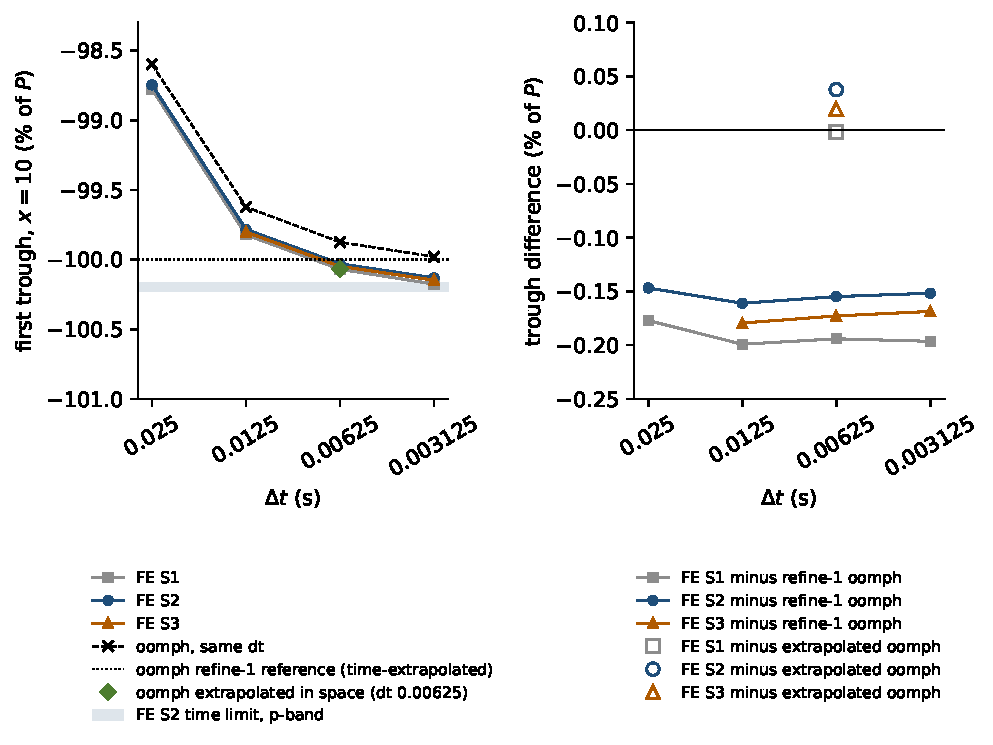
\includegraphics[width=0.72\textwidth]{paper-data/fenicsx_collapsiblechannel/figures/fenicsx_collapsible_trough_time}
\caption{Left: first trough at $x=10$ against $\Delta t$ for the three FE meshes, the oomph-lib same-$\Delta t$ values, the oomph reference and the band of the S2 time limit ($p_\mathrm{ext}=1$ to $2$). Right: FE minus oomph at the same $\Delta t$; the difference does not change with $\Delta t$.}\label{fig:cc_time}
\end{figure}

\section{Model form: an open-loop test}\label{sec:cc_mf}
The oomph wall is a Kirchhoff--Love beam~\citep{Heil2006}, the FE wall a plane-strain continuum, and the dry-wall gap between the two models (preflight) is $0.10$--$0.25\,\%\,P$, unresolved. A preregistered open-loop replay (MF1, amended before the runs) isolates it: the fluid load of one coupled run (S2, $\Delta t=0.00625$, stored at every step as the fluid residual at the interface velocity dofs, normal and shear) is applied as a prescribed dead load (external pressure as follower) to the continuum wall alone and to the oomph-equation beam (Hermite elements, one per $P_2$ wall element).
The replay is interpretable: the rerun reproduces the stored cell to $1.7\times10^{-14}$, and the replayed continuum reproduces the coupled wall history to $1.0\times10^{-7}$ of its maximum (tolerance $10^{-6}$; \texttt{data/mf1\_controls.csv}).
\begin{table}[!htb]
\centering
\caption{MF1: beam (160 elements) minus continuum midplane, same load history (\pP). The last two rows are the FE-minus-oomph same-$\Delta t$ trough differences (S2 and S3, $\Delta t=0.003125$). \texttt{data/mf1\_gap.csv}, \texttt{same\_dt\_offset\_to\_oomph.csv}.}\label{tab:cc_mf}
\small
\begin{tabular}{@{}lrrr@{}}
\toprule
 & $x=7.5$ & $x=10$ & $x=12.5$ \\
\midrule
gap, $\max_t|Y_\mathrm{beam}-d_\mathrm{mid}|$ & 0.053 & 0.033 & 0.056 \\
gap, 80 beam elements & 0.020 & 0.016 & 0.022 \\
gap against the bottom face & 0.076 & 0.040 & 0.078 \\
$V_1$: beam minus continuum & $-0.053$ & $-0.033$ & $-0.056$ \\
$V_1$: FE S2 minus oomph (same $\Delta t$) & $-0.059$ & $-0.152$ & $-0.074$ \\
$V_1$: FE S3 minus oomph (same $\Delta t$) & $-0.085$ & $-0.169$ & $-0.098$ \\
\bottomrule
\end{tabular}
\end{table}
The registered open-loop gap is $0.033$--$0.056\,\%\,P$, inside the limit of $0.15$ (the beam gap \emph{increases} on refinement, $0.016$--$0.022$ at 80 elements to $0.033$--$0.056$ at 160, the two beams differing by $0.033$--$0.049$; 320 elements were not run, so $0.033$--$0.056$ is not a bound). Its sign is opposite to the FE-minus-oomph offset: the beam under the same load is \emph{deeper} than the continuum, whereas oomph-lib (beam) is \emph{shallower} than the FE (continuum). At $x=10$ it is $4.6$ to $6$ times smaller than the offset ($0.033$ against $0.15$--$0.20$); at the quarter points the offset is smaller ($0.05$--$0.11$) and the ratio is only about $0.9$--$2$ (at $x=12.5$ the offset can be smaller than the gap). The offsets above use the bottom face; with the midplane (deeper by $0.007$ at $x=10$, $0.023$ at the quarter points) they are $-0.159$ and $-0.176$ at $x=10$ (S2, S3, $\Delta t=0.003125$) and $-0.08$ to $-0.12$ at the quarter points. There the face convention ($0.02$), the gap ($0.03$--$0.06$) and the offset ($0.05$--$0.12\,\%\,P$) are comparable, so only the \emph{sign} is compared at the quarter points. Hence the wall model form, in an open loop with a dead load, one cell, does not explain the sign or (at mid-span) the size of the offset. This is \textbf{not} a closed-loop result: the pressure--deflection feedback can amplify or attenuate a quasi-static model difference by an unestimated amount, and the load acts at the bottom face (continuum) and on the axis (beam). Not excluded: the oomph spatial-error estimate ($0.26\,\%\,P$, sign unknown), differences in the closed-loop load, shared-definition effects, closed-loop amplification of the gap. The cause of the offset is \textbf{not established}.
\begin{figure}[!htb]
\centering
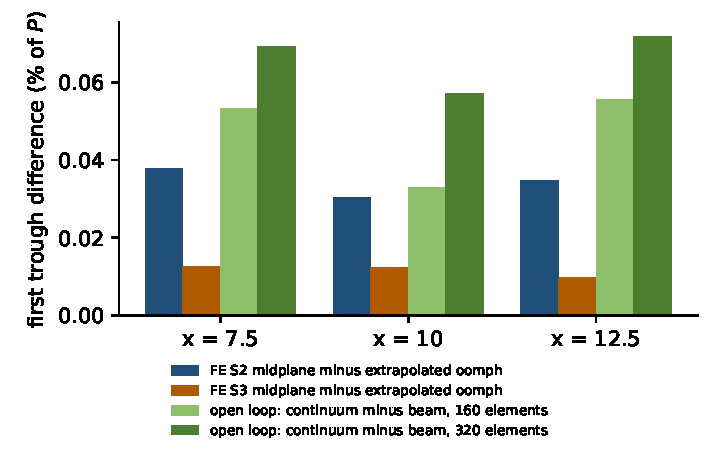
\includegraphics[width=0.38\textwidth]{paper-data/fenicsx_collapsiblechannel/figures/fenicsx_collapsible_model_form}
\caption{Open-loop continuum-minus-beam trough difference (MF1) against the FE-minus-oomph same-$\Delta t$ trough differences, per monitoring point. The signs are opposite at all three points.}\label{fig:cc_mf}
\end{figure}

\section{Comparison with the solids4foam mesh study}\label{sec:cc_s4f}
All solids4foam values here are the F1--F4 runs \legbc{} of the mesh study (PR~\#51; wall midpoint, $x=10$): first trough $-99.841$, $-99.961$, $-100.022$, $-100.048\pP$; the FE value at the same $\Delta t$ ($0.00625$) is $-100.049$ (S3) and $-100.031$ (S2), so the S3 trough differs from F4 by $-0.001\pP$ \uref. The F1--F4 trough changes by $0.21\,\%\,P$ over the four fluid levels, the FE trough by $0.04\,\%\,P$ over S1 to S3 at the same $\Delta t$: at the trough the FE combination is less mesh sensitive than the solids4foam ladder (a statement about the trough value only, not about the histories). History norms at $\Delta t=0.00625$, $x=10$: FE S3 minus F4 has $L_\infty=0.28\,\%\,P$ over $t\le1.25\,\mathrm s$ but $0.40$ over $1.5\,\mathrm s$ (S2: $0.30$, $0.43$) \uref; FE S2 and S3 minus the oomph same-$\Delta t$ run $0.48$ and $0.57$ (F4 minus oomph $0.47$, $0.50$), S1 $0.84$ and $1.26$ (\texttt{data/history\_norms.csv}). The FE and solids4foam error series against oomph-lib are correlated at $0.85$ for S3 and $0.79$ for S2 ($t\le1.25$; $0.83$ and $0.75$ over $1.5\,\mathrm s$; \texttt{data/error\_series\_correlation.csv}).
\paragraph{What this does and does not show about the $0.5\,\%$ floor.}
A third code reproduces a same-$\Delta t$ difference to oomph-lib of the size of the floor (about $0.5\,\%\,P$ in $L_\infty$, S2/S3) \emph{in this restricted sense only}: FE and solids4foam are both plane-strain continuum codes and share a lineage, so a shared difference to a Kirchhoff--Love beam is also what the model-form difference predicts, and the open-loop test above does not remove that possibility in the closed loop. The floor is attributed \textbf{neither to solids4foam nor to oomph-lib}; the same-$\Delta t$ offset of the FE trough is shared with solids4foam F4 \uref. The FE time behaviour matching oomph's (\ref{sec:cc_time}) indicates that temporal error does not account for the constant trough offset. The solids4foam data are one run per level, pre-\#671; no solids4foam time limit is quoted, and the finest S3 cell has no data beyond $1.25\,\mathrm s$.

\section{Formulation controls and gates}\label{sec:cc_ctl}
Stage 3 changed one choice at a time on S2 (change of $V_1$ against the baseline at the same $\Delta t$, \pP{}, maximum over $x$; \texttt{data/stage3\_variants\_vs\_S2.csv}): Newmark wall inertia (FM-N) $\le0.0014$; the tutorial's end conditions (FM5, fixed $p$, zero-gradient $\bm u$) $\le1.4\times10^{-5}$, at the price of exact mass conservation (q-sum $2.5\times10^{-3}$, waived by the preregistration); strict and loose Newton tolerances (NL1, NL2) $<10^{-6}$ and $0.0002$ (q-sum $8.3\times10^{-8}$); two and eight wall rows $0.0053$ and $0.0013$; constant mesh stiffness $<10^{-11}$. The first-order positive controls (backward Euler everywhere, including wall inertia and kinematic row; FM3, FM4) move $V_1$ by $4.84$ and $2.62$ and are detected.

The formulation switches are inert at $\le0.005\,\%\,P$. The trapezoid wall-velocity route (FM-W, hypothesis H4b) was \textbf{not run}. The production gates (mass, pressure parity, force, Jacobian) hold in every cell: weak against direct interface force $\le0.31$, $0.16$, $0.08\,\%$ of the maximum force at S1, S2, S3, balance residual $\le4.6\times10^{-10}\,\mathrm{N/m}$ against forces of $3\,450$--$3\,850\,\mathrm{N/m}$. The BDF-GCL residual is reported, not a pass/fail gate in production, and exceeds the preflight criterion $10^{-6}$ at $\Delta t=0.0125$ and $0.00625$; it is $7.8\times10^{-6}$, $2.1\times10^{-6}$, $5.3\times10^{-7}$ of the maximum volume rate at $\Delta t=0.0125$, $0.00625$, $0.003125$ ($\Delta t^2$ scaling). These are consistency checks of the monolithic form, not physical validation; the solid-side stress-recovered force is not a valid check (several times off) and is not used.

\section{Deviations, failures and what is missing}\label{sec:cc_dev}
Declared deviations from the frozen preregistration: FM-W and WL3 not run; reduced stage-3 grid with parameters chosen after the freeze and before the runs (Amendment~1, written after the stage-1 S1 and S2 cells existed); the S3 cell at $\Delta t=0.003125$ launched before the $0.00625$ cell finished, on its partial rate; S3 primary values over five times for the coarser cells but $t\le1.25\,\mathrm s$ for the finest; FM3/FM4 first order also in wall inertia and kinematic row; job 16869 cancelled for an oversubscribed core and rerun once; the S3 cells at $\Delta t=0.0125$, $0.00625$ started before the Amendment~1 source edit (default path unchanged to about $10^{-14}$ m or better). The preflight failures are in Table~\ref{tab:cc_pre}.
\emph{Not established:} the cause of the offset; a spatial order or limit; the wall resolution separately from the fluid mesh (WL3); a closed-loop beam-versus-continuum result; the kinematic-route sensitivity (FM-W); the solids4foam state under \#671 for the Robin, $\Delta t=0.00625$ runs; independence.

\section{What is claimed and what is not; relation to other contributions}\label{sec:cc_claims}
\begin{itemize}
\item \textbf{Claimed.} A same-lineage monolithic implementation of the tutorial model that runs the $1.5\,\mathrm s$ collapse at three spatial levels and four time steps with the production gates met (the preflight null-state and GCL criteria remain missed); a model-free time-error pattern of the first trough matching oomph-lib's to $0.003$--$0.014\,\%\,P$ \uref; a constant FE-minus-oomph trough offset of about $-0.15$ to $-0.18\,\%\,P$ at $x=10$ that is a limit difference, not temporal truncation; an open-loop model-form gap of $0.033$--$0.056\,\%\,P$ of the opposite sign; no wall-normal pressure-parity mode in $P_2/P_1$.
\item \textbf{Not claimed.} Independent validation; agreement beyond the stated qualifier; a spatial order or limit; the cause of the floor or of the offset; closed-loop model-form equivalence; the effect of \#671 on any solids4foam value; that S1 is history-converged; anything about FEBio. Limitations: one mesh family with tied wall and fluid resolution; one MF1 cell; no external review; private solver and raw data.
\item \textbf{Overlap and added value.} PR~\#30 (FEBio, open) finds a row-parity mechanism, absent here in $P_2/P_1$; PR~\#51 (merged) supplies the solids4foam series of \ref{sec:cc_s4f}; PR~\#45 and the benchmark inventory are unaffected. The added value is modest: a third discretisation shows that the equal-$\Delta t$ comparison of the paper cancels the temporal error at the trough \uref, that the offset does not shrink with $\Delta t$ (exploratory, not preregistered), and gives an open-loop (dead load, one cell) model-form gap of the opposite sign, with the closed loop not estimated; it does not resolve the floor. The authors may reasonably decline any main-text pointer.
\end{itemize}

\section*{AI-use disclosure (placeholder for author review)}
\hl{TBD by the authors:} AI coding and writing assistants (Anthropic Claude) were used to implement and run the FEniCSx code, post-process results, audit them internally and draft this text; the authors are to confirm, edit and take responsibility for the content, and to agree the wording against the journal's policy. No authorship is assigned to an AI system.

\bibliography{bibliography}

\end{document}
